\section{Solver Architecture}

\subsection{Implementation Overview}

The solver is implemented as a modular Python package. Its main modules are summarized in Table~\ref{tab:modules}. The design goal is to keep the numerical core transparent and testable while using sparse linear algebra for consumer-hardware feasibility.

\begin{table}[H]
\centering
\caption{Main solver modules.}
\label{tab:modules}
\begin{tabular}{ll}
\toprule
Module & Responsibility \\
\midrule
\texttt{grid.py} & Axisymmetric grid and indexing convention \\
\texttt{operators.py} & Sparse Laplace/Poisson finite-difference operator \\
\texttt{boundary\_conditions.py} & Dirichlet boundary insertion \\
\texttt{electrostatics.py} & Laplace/Poisson solve entry points \\
\texttt{fields.py} & Electric-field reconstruction and interpolation \\
\texttt{geometry.py} & ImplicitCone with C1 rounded cap-flank geometry \\
\texttt{immersed.py} & Fractional-distance immersed Dirichlet stencils \\
\texttt{interface.py} & Interface geometry, curvature, half-angle extraction \\
\texttt{residual.py} & Young--Laplace--Maxwell residual diagnostics \\
\texttt{space\_charge.py} & Gaussian and threshold space-charge closures \\
\texttt{optimization.py} & Cone-family shape optimization with onset projection \\
\texttt{verification.py} & Immersed verification workflows \\
\texttt{app\_backend.py} & Streamlit-independent backend for interactive app \\
\bottomrule
\end{tabular}
\end{table}

\subsection{Computational Pipeline}

A typical solver run follows this sequence:
\begin{enumerate}
    \item Input physical and numerical parameters, including voltage, surface tension, domain size, and grid resolution.
    \item Build a two-dimensional axisymmetric $(r,z)$ grid.
    \item Construct electrode and boundary masks (or use immersed boundary representation).
    \item Assemble the sparse axisymmetric Laplace/Poisson matrix.
    \item Apply boundary conditions (staircase or immersed Dirichlet stencils) and solve $A\boldsymbol{\ph}=\boldsymbol{b}$.
    \item Reconstruct $\Er$, $\Ez$, and $\Emag$.
    \item Sample a candidate interface $R(z)$ from the ImplicitCone geometry.
    \item Compute interface normals, curvature, Maxwell pressure (from immersed $E_n$ reconstruction), capillary pressure, and residual.
    \item For immersed free-boundary optimization, project out the onset voltage $V_0^*$ per candidate.
    \item Optionally update the space-charge closure and repeat the Poisson solve until convergence.
    \item Return diagnostics, plots, and exported arrays.
\end{enumerate}

\begin{figure}[H]
\centering
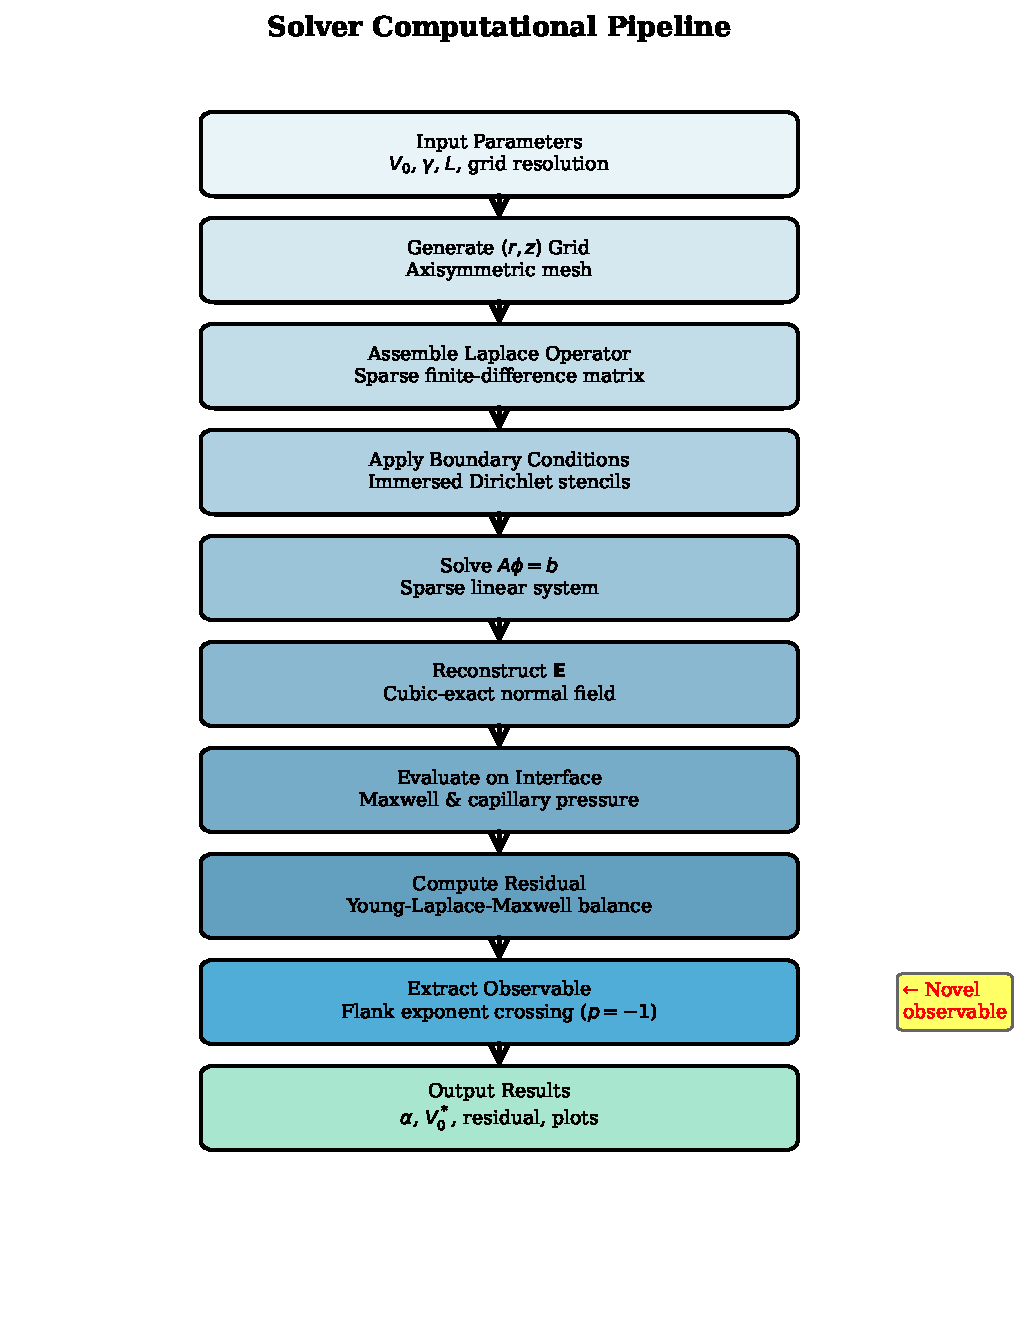
\includegraphics[width=0.7\textwidth]{figures/solver_flowchart.pdf}
\caption{Solver computational pipeline from input parameters to output observables. The flank-field exponent crossing (highlighted) is the novel observable that enables robust angle identification.}
\label{fig:solver-flowchart}
\end{figure}

\subsection{Consumer-Hardware Design}

The solver uses sparse matrices rather than dense matrices. For a grid of $n_r\times n_z$ nodes, the number of unknowns scales as $n_r n_z$, while the finite-difference operator has only a small number of nonzero stencil entries per row. This allows small-to-moderate grids to run quickly on a standard laptop.

\paragraph{Computational Performance.} Solution time scales approximately as $\mathcal{O}(N^{2.3})$ where $N$ is the total number of grid points. A production-quality $121\times177$ grid (21,417 points) solves in approximately 13 seconds on a 2020 MacBook Pro (Apple M1, 8GB RAM). For comparison, equivalent COMSOL Multiphysics simulations with adaptive meshing require approximately 30 minutes on workstation hardware \cite{fernandez2006electrospray}. This performance difference enables rapid parameter studies and real-time interactive exploration during development.

\subsection{Interactive App}

The repository includes a Streamlit application that exposes basic parameters such as voltage, surface tension, electrode spacing, domain radius, grid resolution, and space-charge model. The app has two tabs: a \emph{Classic} tab for the legacy staircase boundary representation, and an \emph{Immersed verification} tab that demonstrates the grounded-box onset-projected optimization and the imposed-Taylor identity verification. It returns scalar diagnostics and Plotly visualizations of potential, electric-field magnitude, space-charge density, interface overlay, and residual profile. The app is a demonstration and analysis interface; the scientific contribution remains the solver and validation workflow.
